\section{Area de estudio}

El estuario del Río de la Plata (RdP) es uno de los sistemas más grandes del mundo ($\approx 3.5 10^{4} km^{2}$) que drena la segunda cuenca más grande de América del Sur luego del Amazonas. Tiene una longitud de 320 km y un ancho de más de 200 km en su boca (Fig. 1.2) y sus aguas son poco profundas ($< 20 m$). Se estima que la cantidad de sedimentos que transporta varía entre 80 y 160 millones de toneladas por año, por lo que es considerado uno de los ríos más turbios del mundo con valores medios de material particulado en suspensión medido en superficie de $100$ a $300$ $mg L^{-1}$ llegando a un máximo de $400$ $mg$ $L^{-1}$ \cite{framinanbrown}. El RdP se caracteriza por la presencia de una zona de máxima turbidez asociada a un frente salino donde se produce el encuentro del agua dulce del río y el agua salada del océano \cite{guerrero1997}\cite{mianzan2001}. La posición de dicho frente está principalmente controlada por la batimetría coincidiendo su posición media con la Barra del Indio en el sector norte y con la isobata de 5 m en la Bahía de Samborombón hacia el sur (Fig. \ref{fig:RdP}). La gran cantidad de sedimentos transportados por el RdP influyen, entre otros, en los procesos sedimentológicos cuyo estudio y comprensión resulta importante para un número de aplicaciones en zonas costeras. Entre ellas pueden mencionarse la evaluación del transporte de sedimentos (optimización de las operaciones de dragado, la comprensión de los cambios batimétricos/línea de costa), el monitoreo de calidad del agua (turbidez), la determinación de profundidad de la capa eufótica para la producción primaria, pesquerías, etc.  


FIGURA 

Dadas las características particulares del RdP, gran superficie y alta concentración de material particulado en suspensión, esta región resulta un área ideal para evaluar y desarrollar algoritmos para la corrección atmosférica que permitan estimar la turbidez o concentración de  material en suspensión a partir de información satelital. En un primer estudio, Dogliotti et al. (2011)\textit{dogliotti2011} analizó en forma cualitativa el desempeño de tres algoritmos de corrección atmosférica aplicados a imágenes MODIS-Aqua en el RdP. Este estudio preliminar mostró que el supuesto de pixel negro en el NIR no se cumple en el RdP debido a la alta concentración de partículas en suspensión, lo que evidencia la necesidad de realizar un análisis cuantitativo con datos radiométricos de campo y evaluar y/o desarrollar algoritmos alternativos. SACARIA LA FIGURA 1.3

\section{Misiones satelitales de color del mar: pasado, presente y futuro}

El primer sensor que midió el color del mar a bordo de un satélite fue el CZCS (\textit{Coastal Zone Color Scanner}), lanzado en el año 1978. A pesar del hecho de que el CZCS fue una misión experimental destinada a durar un año, el sensor continuó generando una serie temporal de datos muy valiosos que permitieron por primera vez observar sinópticamente la distribución espacial y temporal de la distribución de la concentración de clorofila (utilizada como indicador de biomasa) en distintas regiones del mundo, y también ha permitido estimar la producción primaria a escala global (Longhurst et al. 1995). Diez años pasaron antes de que otros sensores destinados a proveer datos de color del mar orbitasen nuevamente alrededor de la Tierra. En particular, el SeaWiFS (\textit{Sea-viewing Wide Field-of-view Sensor}), lanzado en 1997 a bordo del satélite SeaStar de la NASA, fue el que interrumpió esta década sin disponibilidad de datos, y produjo datos hasta el 2010. Algunos de los sensores posteriores más destacados fueron los MODIS (\textit{Moderate-resolution Imaging Spectroadiometer}) a bordo de los satélites Aqua y Terra (actualmente en funcionamiento), y el MERIS (\textit{MEdium Resolution Imaging Spectrometer}) a bordo del satélite Envisat de la Agencia Espacial Europea (ESA) que fue lanzado en el 2002 dejó de ser operacional desde el 2012. Otros sensores destinados a color del mar fueron lanzados mas recientemente, incluyendo el OCM-2 (\textit{Indian Ocean Colour Monitor}), el GOCI (\textit{Korean Geostationary Ocean Color Imager}, el primer sensor geoestacionario destinado a color del mar) y el VIIRS (\textit{Visible Infrared Imager Radiometer Suite }). Nuevos sensores de color del mar están planeados dentro de la siguiente década por varias agencias espaciales, entre ellas puede mencionarse el sensor OLCI (Ocean Land Colour Instrument) que será lanzado a bordo del Sentinel-3 por la ESA, la misión PACE (Pre-Aerosol, Clouds and ocean Ecosystem) que será lanzada por la NASA y la misión Argentina-Brasilera SABIA-Mar.
La Comisión Nacional de Actividades espaciales (CONAE) en conjunto con la Agencia Espacial Brasileñna (AEB) y el Instituto Nacional de Desarrollos Espaciales de Brasil (INPE) se encuentran actualmente desarrollando la misión SABIA-Mar (SAtélite Argentino Brasileño par ala Información del Mar). El principal objetivo de la misión es proveer información y productos para el estudio de los ecosistemas marinos, el ciclo del carbono, la cartografía de costas y hábitats marinos, peligros en el litoral marino, aguas continentales y las actividades pesqueras (CONAE, 2013). 
Los sensores ópticos del SABIA-Mar tendrán bandas espectrales compatibles con los sensores SeaWiFS, MODIS y MERIS. SABIA-Mar contará con una resolución de 200 m en las áreas de interés específico que constituyen las zonas costeras y marítimas de Argentina y Brasil, como así también las aguas continentales de América del sur. Y una resolución de 1 km para estudios regionales y de cobertura global del océano con el fin de mantener una continuidad y compatibilidad con las demás misiones de color. Según se encuentra actualmente planeada la misión, el SABIA-Mar contará con las mismas bandas que el MODIS para la corrección atmosférica (tanto en el NIR como en el SWIR) mas una banda que también ha sido incorporada en el sensor OLCI (1020 nm) que podría ser utilizada tanto para la corrección atmosférica como para la estimación de la concentración de material particulado en suspensión en aguas turbias (CONAE, 2013; Knaeps et al. 2012). 

\section{Objetivos}

La propuesta de tesis planteada propone como objetivo general contribuir en el conocimiento para mejorar la corrección atmosférica en aguas turbias, con especial interés en las aguas del Río de la Plata, mediante simulaciones y datos de campo. El trabajo planteado se encuentra en el marco y contribuirá en forma directa a la misión Argentina-Brasilera SABIA-Mar ya que las simulaciones fueron realizadas para un sistema satélite-sensor con las características del propuesto para dicha misión. Con el fin de alcanzar el objetivo general se plantearon los siguientes objetivos específicos:

- Simular la reflectancia al tope de la atmósfera en las bandas espectrales ubicadas en la región NIR y SWIR del sensor SABIA-Mar teniendo en cuenta diferentes geometrías de observación e iluminación del SABIA-Mar, de condiciones atmosféricas y reflectancias de aguas turbias en general y esperables en la región del Río de la Plata obtenidas a partir de simulaciones y datos de campo.

- Implementar un modelo inverso semi-empírico para estimar la reflectancia del agua en la región NIR del espectro (rhow(865)) basado en componentes principales.

- Evaluar teóricamente el desempeño del modelo inverso para estimar rhow(865) utilizando diferentes combinaciones de bandas y para aguas con diferente características reflectivas (cantidad de material particulado).

\chapter{Marco físico}
\label{ch:marcofisico}

En este capítulo se presentan las herramientas y los conceptos
físicos y matemáticos que serán utilizados en los capítulos siguientes. Más específicamente:
\begin{enumerate}
\item Se definen los ángulos pertinentes a la geometría de observación-iluminación.
\item Se definen algunos términos radiométricos, tales como la irradiancia,
la radiancia, la reflectancia y en particular se definirá lo que comúnmente se llama
en teledetección el \textit{color del mar};
\item Se presenta la Teoría de Transferencia Radiativa, las hipótesis bajo las cuales trabaja, y
la \textit{ley de Boguer-Lambert-Beer} para establecer el balance de energía radiativa en ausencia de polarización, conocido como \textit{ecuación escalar de transferencia radiativa};
\item Se generaliza al caso en que sí se tiene en cuenta la polarización de la radiación: la
\textit{ecuación vectorial de transferencia radiativa}, que es de donde parte el código de
transferencia radiativa (código SOS) utilizado en el presente trabajo;
\item Se describen las diferentes componentes que influyen en la radiación que llega
al sensor, tales como la presencia de la atmósfera y los efectos que ocurren en
la interfase del mar y en el seno del cuerpo de agua debido a las distintas sustancias presentes;
\end{enumerate}

\section{Magnitudes físicas básicas en teledetección}
\label{ch:marcofisico:magnitudes}
%%%%%%%%%%%%%%%%%%%%%%%%%%%%%%%%%%%%%%%%%%%%%%%%%%%%%%%
El sensoramiento remoto o la \textit{teledetección} es una técnica que permite adquirir
información mediante el análisis de datos colectados por instrumentos que no
están en contacto físico con los objetos investigados. Los sensores remotos,
generalmente a bordo de aviones o satélites que orbitan la Tierra, miden la energía
o radiación electromagnética (REM) que es reflejada o emitida por los objetos. Dicha radiación
es cuantificada a partir de varias magnitudes físicas, entre las cuales
están la irradiancia, la radiancia y la reflectancia, definidas a continuación. Se asumirán
escenarios con campos de radiación estacionarios, por lo que se omitirá la dependencia del tiempo de las
magnitudes presentadas.

\subsection{Variables geométricas de observación-iluminación}
Previo a introducir las magnitudes radiométricas, es necesario definir la convención usual utilizada en teledetección para determinar las direcciones de incidencia solar y de observación.
En la Fig.\ref{fig:obs_ilum} se esquematiza el sistema sol-sensor en conjunto con los ángulos asociados a la geometría de observación-iluminación.
 
\begin{figure}
\centering
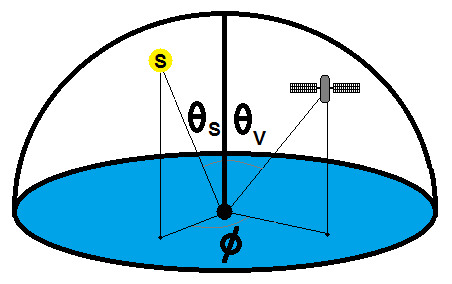
\includegraphics[width=0.65\textwidth]{obs_ilum}
\caption[Geometría de observación-iluminación]{Definición de los ángulos cenitales ($\t$) y acimutales ($\p$) solar y de observación (subíndices $S$ y $V$, respectivamente.),
según la convención generalmente utilizada en teledetección.} 
\label{fig:obs_ilum}
\end{figure}

En general en teledetección se define la dirección en la cual se propaga la radiación en coordenadas
esféricas, tomando como dirección polar el cenit; por lo que $\t$ representa el ángulo cenital. El ángulo acimutal $\p$ se mide desde el plano principal en sentido antihorario respecto del cenit,
es decir, asumiendo un ángulo cenital solar $\p_{S}=0$. En el esquema de la Fig. \ref{fig:obs_ilum},
se determinan las dos direcciones más pertinentes: la del limbo solar y la de observación. En las
definiciones dadas a continuación, donde aparezca la dupla $(\t,\p)$, esta referirá a una dirección
campo genérica, que podrá ser identificada con la dirección en que se halle el sensor, $(\t_{V},\p_{V})$.

\subsection{Irradiancia}
Considérese un flujo de energía radiativa atravesando un diferencial $dS$ de
superficie plana. La tasa de flujo de energía radiativa, o potencia,
por unidad de superficie se denomina
\textit{irradiancia}, $E$, y es expresada en términos de energía neta
$d^{2}U$ que atraviesa la superficie $dS$ en el intervalo temporal $[t,t+dt]$, o bien
la potencia neta $d\Phi$ o \textit{flujo radiante} que atraviesa la superficie $dS$ como

\begin{equation}
 E=\frac{d^{2} U}{dS\,dt}=\frac{d\Phi}{dS}\quad [W \cdot m^{-2}]
\label{irradiancia}
\end{equation}

La cantidad $d\Phi$ es diferencial de primer orden,
considerada \textit{positiva} si el flujo radiante egresa del hemisferio superior
(ascendente, $u$, suponiendo que la superficie sea horizontal)
y \textit{negativa} en caso contrario (descendente, $d$).
Es conveniente separar el flujo radiante en dos aportes positivos
según si es ascendente o descendente, $d\Phi_{u}$ y $d\Phi_{d}$,
cada uno de los cuales aporta una cantidad positiva de energía.
Las irradiancias ascendente y descendente se definen entonces como

\begin{equation}
 E_{u}=\frac{d\Phi_{u}}{dS}, \quad
 E_{d}=\frac{d\Phi_{d}}{dS}\quad [W\cdot m^{-2}]
\label{irrad_ascen_descen}
\end{equation}

El flujo radiante neto en la dirección ascendente es $d\Phi=d\Phi_{u}-d\Phi_{d}$.
De la misma manera, la irradiancia neta es escrita como la diferencia entre dos cantidades positivas:
$E=E_{u}-E_{d}$, siendo estas las medidas de toda la REM que sale y llega a una
superficie, respectivamente (Fig. \ref{fig:dogliotti1}).

\begin{figure}
\centering
\includegraphics[width=0.6\textwidth]{dogliotti1}
\caption[Irradiancias ascendente y descendente]{Geometría asociada a la definición de irradiancia descendente ($E_{d}$) y ascendente ($E_{u}$),
donde $d\Phi$ es el flujo radiante que llega a la superficie $dS$.} 
\label{fig:dogliotti1}
\end{figure}

\subsection{Radiancia}
Los sensores remotos tienen un campo limitado de observación y no reciben toda
la irradiancia emitida por una superficie debido a que la forma del detector y su
geometría de observación limitan la señal a una pequeña fracción del flujo. Por lo
tanto es necesario tener una descripción de la variación del flujo en función de la
dirección: esto se podrá hacer fácilmente dado que los rayos que se trasladan en 
diferentes direcciones no interactúan, por lo que se podrán tratar separadamente.

Considérese entonces un flujo radiante $d^{2}\Phi$ dentro de un ángulo sólido
$d\Omega$ alrededor de la dirección $\hat{\Omega}$, atravesando un diferencial
de superficie plana $dS$ (e.g. la superficie de un colector \textit{plano})
cuya orientación queda determinada por su normal $\hat{z}$ (ver Fig. \ref{fig:dogliotti2}).
El ángulo comprendido entre $\hat{z}$ y la dirección de propagación $\hat{\Omega}$ es $\t$. 
La potencia por unidad de superficie y por unidad de ángulo sólido se denomina \textit{radiancia}, $L(\t,\p)$,
y viene dada por:

\begin{equation}
 L(\t,\p)=\frac{d^{2}\Phi}{cos\,\t\,dS\,d\Omega}\quad [W\cdot m^{-2} \cdot sr^{-1}]
\label{radiancia}
\end{equation}

Nótese que, además de haber dividido por $d\Omega dS$, se ha dividido por el factor
$cos \t=\hat{z}\cdot \hat{\Omega}$, es decir, la proyección del elemento de superficie al plano
normal a $\hat{\Omega}$.
Es por esto que un colector de radiación plano se denomina \textit{colector coseno}.
Nótese también que si $\hat{z}$ y $\hat{\Omega}$ apuntan en hemisferios opuestos,
entonces $\hat{z}\cdot \hat{\Omega}$ es negativo.
El flujo radiante es también negativo en este caso, por definición; por lo que la relación
$d^{2}\Phi/cos(\t)$ se mantiene positiva: \textit{la radiancia es siempre positiva}.
En la figura \ref{fig:dogliotti2} se muestra la geometría asociada a la radiancia.

\begin{figure}
\centering
\includegraphics[width=0.6\textwidth]{dogliotti2}
\caption[Radiancia]{Geometría asociada a la definición de radiancia, donde $dS$ es
el área de un elemento de la superficie, $L(\t,\p)$ es la radiancia que sale de $dS$
con un ángulo cenital $\t$ (relativo a la normal de la superficie) y un ángulo acimutal $\phi$.
Su valor es definido por el flujo
radiante que sale de $dS$ dentro del ángulo sólido $d\Omega$,
centrado en la línea definida por $\theta$ y $\phi$.} 
\label{fig:dogliotti2}
\end{figure}

Se obtendrá la relación entre radiancia e irradiancia a partir de la Ec. \eqref{radiancia}, que se podrá reescribir como

\begin{equation}
 d^{2}\Phi=L(\t,\p)cos(\t) dS d\Omega
\label{radiancia_bis}
 \end{equation}

Utilizando las Ecs. \eqref{irradiancia} y \eqref{radiancia_bis} se obtienen
las siguientes relaciones entre irradiancias (ascendente y descendente) y radiancia:

\begin{equation}
 E_{u}=\frac{d\Phi_{u}}{dS}=\int_{u}d\Omega L(\t,\p)cos(\t),\quad  E_{d}=\frac{d\Phi_{d}}{dS}=\int_{d}d\Omega L(\t,\p)cos(\t)
\label{rad_irrad1}
 \end{equation}

Sendas magnitudes son definidas positivas. Combinándolas, se obtiene que \textit{la irradiancia es
la integración de $L(\t,\p)cos(\t)$ sobre todo el ángulo sólido},

\begin{equation}
 E=E_{u}-E_{d}=\int_{4\pi}d\Omega L(\t,\p)cos(\t)\quad [W\cdot m^{-2}]
\label{rad_irrad2}
 \end{equation}

Obsérvense dos casos límite en la distribución angular de la radiancia a partir de las dos situaciones propuestas a continuación: 

\begin{enumerate}
\item \textbf{Radiancia proveniente del limbo solar}. En caso de despreciar el ángulo sólido abarcado por el limbo solar en el cielo terrestre, la radiancia solar incidente, previa a interactuar con la atmósfera, puede ser escrita como

\begin{equation}
L_{S}(\t,\p)(\hat{\Omega})=E_{S}\delta(\hat{\Omega}-\hat{\Omega}_{S})
\label{limbosolar}
 \end{equation}

siendo $\hat{\Omega}_{S}=(\ts, \ps=0)$ la dirección en la que se halla el limbo solar, $\delta(\hat{\Omega}-\hat{\Omega}_{S})=\delta(\p)\delta(cos \t - cos \t_{S})$ la distribución delta de Dirac bidimensional, y $E_{S}$ la irradiancia solar extraatmosférica (véase. Fig. \ref{fig:thuillier}).

\item \textbf{Radiancia saliente de una superficie lambertiana.}

En caso de incidir sobre una superficie horizontal que sea un difusor perfecto,
o sea una superficie que emite o refleja la
energía con la misma intensidad en todas las direcciones independientemente del
ángulo con el que incide la radiación, tendríamos, en las cercanías de la misma, siguiendo la Ec. \eqref{rad_irrad1},

\begin{equation}
 E_{u}=E_{d}=\pi L
\label{superficielambertiana}
 \end{equation}

A este tipo de superficies se las llama \textit{lambertianas} (Fig. \ref{fig:dogliotti4}a). 
Ninguna superficie es perfectamente lambertiana, pero muchas de ellas, especialmente las opacas, se aproximan bastante. Como caso opuesto a una superficie lambertiana puede mencionarse la superficie especular (Fig. \ref{fig:dogliotti4}b). En este tipo de superficie la energía es reflejada con un ángulo igual al incidente pero en sentido opuesto. Las superficies naturales en general se comportan de forma intermedia (Fig. \ref{fig:dogliotti4}c).

\begin{figure}[H]
\centering
\includegraphics[width=0.75\textwidth]{dogliotti4}
\caption[Tipos de superficies reflectoras]{Diferentes tipos de reflexión: (a) difusa o lambertiana, (b) especular y (c) tipo mixta.} 
\label{fig:dogliotti4}
\end{figure}
\end{enumerate}

\subsection{Reflectancia y \textit{color del mar}}
Todas las propiedades ópticas del agua varían con la longitud de onda ($\l$), por lo tanto se definen la irradiancia espectral ($E(\l)$) y la radiancia espectral ($L(\l,\t,\p)$) de manera análoga pero considerando radiación en el rango espectral diferencial $[\l,\l+d\l]$, es decir:

\begin{align}
 &E(\l)=\frac{d E}{d\l}(\l) \quad [W m^{-2} \mu m^{-1}] \\
 &L(\l,\t,\p)=\frac{d L}{d\l}(\l,\t,\p) \quad [W m^{-2} sr^{-1} \mu m^{-1}]
\label{lambertiana}
 \end{align}

El \textit{color intrínseco del mar} está determinado por la variación espectral de la
reflectancia superficial $\rho_{W}(\l)$. La reflectancia irradiante está definida como la relación
entre la irradiancia ascendente ($E_{u}$) y la irradiancia descendente ($E_{d}$), justo por encima del agua ($z=0^{+}$), o sea:

\begin{equation}
\rho_{W}(\l)=\frac{E_{u}(\l,z=0^{+})}{E_{d}(\l,z=0^{+})} \quad [s/u]
\label{reflectancia}
\end{equation}

De esta magnitud se parte para la estimación de las diferentes sustancias presentes en el agua. Algunas firmas de reflectancias del agua pueden verse en la Figs. \ref{fig:rios} y \ref{fig:casoIyII}.

\section{Teoría de transferencia radiativa para una atmósfera plano-paralela}
En esta sección, se describirá cómo es el flujo de energía radiativa a través de la atmósfera y los océanos según la Teoría de Transferencia Radiativa (TTR). Por el momento, se ignorarán los efectos de polarización, lo que significa que se despreciarán las componentes $Q$, $U$ y $V$ del vector de Stokes.
Este enfoque se denomina la \textit{aproximación escalar}, en contraste con la descripción \textit{vectorial}, más precisa, que detallaremos más adelante.
En general, esta aproximación es válida para radiación de onda larga donde la emisión térmica
y la absorción son más importantes. Sin embargo, a longitudes de onda más cortas (e.g. la región
visible del espectro), donde la dispersión es importante, la radiación está parcialmente polarizada, generalmente. La polarización es parte esencial en la descripción de la dispersión de la luz solar en una atmósfera clara o en agua pura (Dispersión de Rayleigh). Generalmente, en las longitudes de onda más cortas, existe un acople entre las diferentes componentes del vector de Stokes, y se requiere considerar la versión vectorial para obtener resultados más precisos. Más adelante, se presentará la versión vectorial, que es la que rige los cálculos realizados por el código de transferencia radiativa SOS utilizado en el presente trabajo; pero es más sencillo generalizarla a partir del caso escalar.

\subsection{Aproximación de la óptica geométrica}
Las asunciones básicas de la TTR son esencialmente las mismas que las de la óptica geométrica. De hecho, en caso de no haber procesos de dispersión o emisión térmica, la ecuación de transferencia radiativa se reduce a la ley de intensidad de la óptica geométrica. La propagación de la REM podrá ser descrita entonces en términos puramente geométricos y el transporte de energía ocurrirá a lo largo de la dirección de los \textit{rayos} de luz. En la óptica geométrica, la difracción y la interferencia de la luz son despreciables, lo mismo ocurrirá en la TTR.

\subsection{Aproximación del índice de refracción}
\label{ch:marcofisico:aproxindrefrac}
Estos rayos de luz no son necesariamente rectos; sino que tienen una curvatura dependiente del \textit{índice de refracción del medio}, $m(\l)$. La parte real de $m(\l)$ es la razón entre las velocidades de propagación en el vacío y la del medio correspondiente, y la imaginaria representa la absorción del mismo. La dependencia de $m(\l)$ con la longitud de onda se conoce también como fenómeno de \textit{dispersión}. Para el sensoramiento remoto en medios acuáticos, en caso de que no se esté considerando REM que haya atravesado la atmósfera de manera muy oblicua (i.e. $\ts$ y/o $\to$ altos),
es aceptable establecer el índice de refracción constante para el aire y para el agua; más específicamente, $m_{AIRE}\approx 1$ y $m_{H_{2}O}\approx 1.334$.

\subsection{La ley de Boguer-Lambert-Beer}
\label{ch:marcofisico:boguerlambertbeer}
Considérese un peque\~no volumen $dV$ conteniendo materia \textit{ópticamente activa}, descrita por la concentración numérica $n$ $[m^{-3}]$. Por practicidad, $dV$ será considerado una lámina de base $dA$ y profundidad $dS$ (Fig.\ref{fig:extincion}). Supongamos que un haz de radiación incide normalmente en el medio. El diferencial de energía con que el haz incide viene dado por la Ec. \eqref{radiancia},

\begin{equation}
d^{2}\Phi=L(\l)\,dS\,dt\,d\l \,d\omega
\label{laambertdif1}
\end{equation}

A medida que el haz atraviesa la rodaja de materia, interactúa con las partículas ya sea a través de la absorción o la dispersión; por lo que una cantidad reducida de energía emerge del lado opuesto. Se dice que el haz sufrió un proceso de \textit{extinción}.

\begin{figure}[H]
\centering
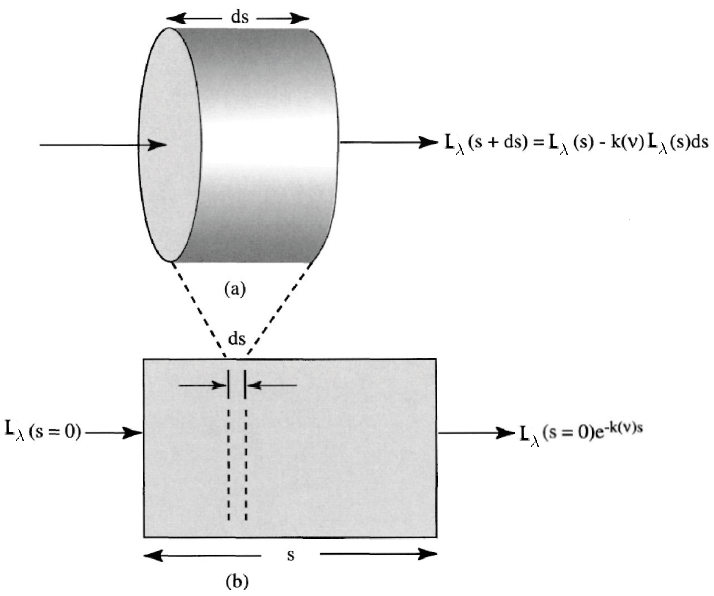
\includegraphics[width=0.6\textwidth]{extincion}
\captionof{figure} [Esquemas de extinción de la luz]{a) La radiación que pasa a través de una rodaja diferencial de materia ópticamente
activa sufre una extinción proporcional al camino diferencial recorrido $ds$.
b) La extinción es exponencial cuando la radiación atraviesa un camino finito $s$ dentro del material.} 
\label{fig:extincion}
\end{figure}

Se encuentra experimentalmente que el grado de decaimiento de la radiancia en un camino diferencial depende linealmente de la radiancia incidente ingresante $L(\l)$ y del camino $ds$ atravesado dentro del material:

\begin{equation}
dL(\l)\propto -L(\l) ds
\label{laambertdif2}
\end{equation}

Dicha ecuación no es más que la versión diferencial de la ETR en que no se considera la presencia de fuentes. La constante de proporcionalidad correspondiente se denomina \textit{coeficiente de extinción del medio}, $\sigma(\l)$. Ahora bien, dado que se está trabajando sobre una atmósfera plano paralela, las propiedades ópticas del sistema de estudio son únicamente dependientes de la altura; por lo que es válido reemplazar:

\begin{equation}
ds=\frac{dz}{\mu}
\label{z_y_s}
\end{equation}

siendo $\mu=cos \t$, con lo que se obtiene la versión diferencial de la \textit{ecuación de Lambert-Boguer-Beer} para una atmósfera plano-paralela:

\begin{equation}
\mu \frac{d L(\l)}{dz}=-\sigma(\l) L(\l)
\label{lambertdif3}
\end{equation}

Integrando la Ec. \eqref{lambertdif3} por separación de variables, tras considerar la Ec. \eqref{z_y_s}, se obtiene:

\begin{equation}
L(\l)(z)=L(\l)(0)e^{-\int_{0}^{z}\frac{dz'}{\mu} \sigma(z,\l)}=L(\l)(0)e^{-\frac{\tau(z,\l)}{\mu}}
\label{lambertint}
\end{equation}

donde se definió la \textit{profundidad óptica} $\tau(z,\l)$ del camino $z$, que podrá despejarse a partir de la Ec. \eqref{lambertint}:

\begin{equation}
\tau(\l,z)=-ln \left( \frac{L(\l,z'=0)}{L(\l,z'=z)} \right) \quad [s/u]
\label{tau_definicion}
\end{equation}

Tanto $\sigma(\l)$ como $\tau(\l)$ pueden ser divididos en su componente debida a la absorción (a) y a la dispersión (s):

\begin{align}
 &\sigma(\l)=\sigma_{a}(\l)+\sigma_{s}(\l)\\
 &\tau(\l)=\tau_{a}(\l)+\tau_{s}(\l)
\label{abs+sca}
 \end{align}

Diferenciando la Ec. \eqref{tau_definicion} respecto de la altura $z$, se halla la siguiente relación biyectiva $\tau\leftrightarrow z$:

\begin{equation}
d\tau=\mu \frac{dL}{L}=-\sigma(z) dz
\label{tau_y_z}
\end{equation}

Dicha biyección permitirá utilizar la profundidad óptica medida desde el TOA hasta $z$ como variable de altura. Obsérvese que $\tau$ aumenta hacia abajo, lo que explica el signo negativo en Ec. \eqref{tau_y_z}. El TOA corresponde a $\tau=0$ y llamaremos $\tau^{*}$ al espesor óptico en la superficie, es decir, el espesor óptico total de la atmósfera. Por lo que la Ec. \eqref{lambertdif3} podrá ser reescrita como:

\begin{equation}
\boxed{\mu \frac{d L(\l)}{d\tau}=L(\l)}
\label{LAMBERT_BEER}
\end{equation}

que será la versión de la ley de extinción sobre la cual se basará la ETR escalar.

\subsection{La ecuación escalar de transferencia radiativa}
\label{ch:marcofisico:EETR}

La ecuación de Boguer-Lambert-Beer tiene en cuenta la absorción y la dispersión como procesos de extinción de un haz de radiación; pero no contempla el hecho de que la luz dispersada por las partículas en la atmósfera y la proveniente de la superficie terrestre sirve también de fuente de REM en esa y otras direcciones. Para poder agregar el término de fuente a la Ec. \eqref{LAMBERT_BEER} es necesario aún presentar dos magnitudes físicas más: la primera es el \textit{albedo de dispersión simple}, $\omega$: 

\begin{equation}
 \omega=\frac{\sigma_{s}}{\sigma}
\label{lenoble2}
 \end{equation}

que representa la fracción de fotones que al interactuar con una partícula sufre un proceso de dispersión respecto de la totalidad de procesos considerados, es decir, absorción y dispersión. 
\footnote{Se asumen como despreciables, aquí y en el resto del presente trabajo, todos los eventos asociados a procesos de dispersión inelástica dada su baja incidencia en las bandas consideradas en este trabajo.}
 
La segunda es la \textit{función de fase}, $p(\Theta)$, que describe la probabilidad de dispersión en función del ángulo $\Theta$, comprendido entre las direcciones incidente y de dispersión. $p(\Theta)$ está normalizada a $4\pi$ cuando se la integra sobre todo el ángulo sólido.

Tomando la Ec.\eqref{LAMBERT_BEER}, agregando la dependencia de las magnitudes con la dirección, y asumiendo la presencia de fuentes, se arriba a la ecuación de transferencia radiativa escalar:

\begin{equation}
\boxed{\mu \frac{d L(\l,\tau,\mu,\phi)}{d\tau}=L(\l,\tau,\mu,\phi)+S(\l,\tau,\mu,\phi)}
\label{EETR}
\end{equation}

donde $S(\l,\tau,\mu,\phi)$ es la \textit{función fuente}, y la misma viene dada por:

\begin{equation}
\begin{split}
S(\l,\tau,\mu,\phi) =&\frac{\omega(\tau)}{4 \pi} 
p(\l,\tau,\mu,\phi,\mu_{S},\phi_{S}) E_{S} e^{-\frac{\tau}{\mu_{S}}} 
+\\ &\frac{\omega(\tau)}{4 \pi} \int_{0}^{2\pi} 
\int_{-1}^{1} p(\l,\tau,\mu,\phi,\mu',\phi') L(\l,\tau,\mu',\phi')d\mu'd\phi'
\end{split}
\label{fuente_escalar}
\end{equation}

donde se han incluido el término asociado a la luz solar directa y el asociado a radiación proveniente de procesos de dispersión.

\subsection{Los parámetros de Stokes}
\label{ch:marcofisico:stokes}

Dado que los procesos de dispersión dependen del estado de polarización, y la modifican, la radiancia derivada a partir de la ecuación escalar (Ec. \eqref{EETR}) es una aproximación que puede diferir del valor exacto hasta en un $10$ \%. Es por esto que se utilizarán los parámetros de Stokes, que contienen información del estado de polarización de la radiación.

Una onda electromagnética viajando en la dirección $\bf{k}$ es caracterizada por las componentes complejas $E_{l}$ y 
$E_{r}$ del campo eléctrico $\bf{E}$, correspondientes a las proyecciones en los versores ortogonales $\bf{l}$ y $\bf{r}$
contenidos en el frente de ondas (de forma tal de que $(\bf{l},\bf{r},\bf{k})$ conforma una terna derecha), o por cualquier combinación de los cuatro parámetros $E_{l}\hat{E}_{l}$, $E_{r}\hat{E}_{r}$, $E_{r}\hat{E}_{l}$ y $E_{l}\hat{E}_{r}$, donde
$\hat{E}$ representa el valor conjugado de $E$. Los parámetros de Stokes quedan definidos por

\begin{equation}
\begin{bmatrix} 
I \\ Q \\ U \\ V 
\end{bmatrix}
=\frac{\epsilon_{0}c}{2}
\begin{bmatrix}
\left<{E_{l}\hat{E}_{l}}\right>+\left<{E_{r}\hat{E}_{r}}\right>\\
\left<{E_{l}\hat{E}_{l}}\right>-\left<{E_{r}\hat{E}_{r}}\right> \\
\left<{E_{l}\hat{E}_{r}}\right>+\left<{E_{r}\hat{E}_{l}}\right> \\
i\left<{E_{l}\hat{E}_{r}}\right>-i\left<{E_{r}\hat{E}_{l}}\right> 
\end{bmatrix}
=\frac{\epsilon_{0}c}{2}
\begin{bmatrix}
\left<{E_{l0}^{2}}\right>+\left<{E_{r0}^{2}}\right>\\
\left<{E_{l0}^{2}}\right>-\left<{E_{r0}^{2}}\right>\\
2\left<{E_{l0}E_{r0}cos(\delta)}\right>\\
2\left<{E_{l0}E_{r0}sin(\delta)}\right>
\end{bmatrix}
\label{lenoble5}
\end{equation}

donde $E_{l0}$ y $E_{r0}$ son las amplitudes de $E_{l}$ y $E_{r}$, respectivamente, y $\delta$ es la fase de retardación
de $E_{l}$ respecto de $E_{r}$; $c$ es la velocidad de la luz en el vacío y $\epsilon_{0}$ la constante dieléctrica del
vacío. Dado que las mediciones siempre incluyen grandes números de trenes de ondas, las cantidades $\left<{x}\right>$
son los promedios temporales de $x$ (en caso de ser ondas monocromáticas, vale, en este contexto, que $\left<{x}\right>=x$).
Los parámetros de Stokes contienen toda la información del campo de radiación. $I$ es la energía total de radiación, 
es decir, equivalente a la irradiancia $E$, o la radiancia $L$, consideradas en la sección anterior. Los otros tres parámetros
tienen las mismas dimensiones que $I$ ($W/m^{-2}$ o $W/m^{-2}sr^{-1}$, según la ocasión); sirven para caracterizar el estado 
de polarización. El mismo es determinado por $\delta$ y por la razón $a=\frac{E_{l0}}{E_{r0}}$. Para una mezcla de
trenes de onda incoherentes, con las mismas amplitudes promedio, $Q=U=V=0$, entonces la radiación es natural o 
no polarizada. Este es el caso de la radiación solar extraatmosférica. Dada la aditividad de los parámetros de Stokes, cualquier haz puede ser analizado como la superposición incoherente de
radiación polarizada con una intensidad

\begin{equation}
 I_{pol}=(Q^{2}+U^{2}+V^{2})^{1/2}
\label{lenoble6}
 \end{equation}

y radiación natural; siendo el grado de polarización:

\begin{equation}
P=I_{pol}/I
\label{lenoble7}
\end{equation}

Para polarización lineal, $\delta=0$ y $V=0$, y $Q$ y $U$ fijan la dirección de polarización.
Si $\alpha$ es el ángulo de rotación alrededor de $\bf{k}$ que alínea $\bf{l}$ a $\bf{E}$, se tienen

\begin{equation}
Q=I_{pol}cos(2\alpha)\quad
U=I_{pol}sin(2\alpha)
\label{lenoble8}
\end{equation}

Para luz elípticamente polarizada, el parámetro $V$ define la elipticidad de la luz polarizada; $V$ es generalmente muy chico en la atmósfera y es usualmente despreciado, por lo que el estado de polarización puede ser considerado lineal.

La radiancia (irradiancia), cantidad usualmente escalar, será convenientemente reemplazada por el vector radiancia (irradiancia), construido a partir de los parámetros de Stokes:

\begin{equation}
 \bf{L}=(I,Q,U,V)^{T}
\label{lenoble9}
 \end{equation}

donde $\bf{x}^{T}$ representa el transpuesto del vector $x$.

\subsection{La matriz de fase}
\label{ch:marcofisico:matrizdefase}

Para poder describir el fenómeno de dispersión considerando el estado de polarización, se deberá reemplazar la función de fase escalar, $p(\Theta)$, por una matriz de $4 \times 4$.

Se elegirán los ejes de referencia $(\bf{l'},\bf{r'})$ y $(\bf{l},\bf{r})$, para la radiación incidente y dispersada en dirección paralela ($\bf{l}$) y perpendicular ($\bf{r}$) al plano de dispersión, definido por las direcciones de incidencia y dispersión. Para una distribución de partículas orientadas al azar, en igual cantidad que sus respectivos quirales (partículas espejadas), condición no muy restrictiva para los aerosoles, la matriz de fase queda, a partir de la teoría de Mie\cite{mischenko}, en la forma:

\begin{equation}
\bf{P}(\Theta)=
\begin{bmatrix}
{P_{11}(\Theta)}&{P_{12}(\Theta)}&{0}&{0} \\
{P_{21}(\Theta)}&{P_{22}(\Theta)}&{0}&{0} \\
{0}&{0}&{P_{33}(\Theta)}&{P_{34}(\Theta)}\\
{0}&{0}&{P_{43}(\Theta)}&{P_{44}(\Theta)}\\
\end{bmatrix}
\label{lenoble10}
\end{equation}

donde $P_{21}=P_{12}$ y $P_{43}=-P_{34}$, y el elemento $P_{11}(\Theta)$ es idéntico a la función de fase $p(\Theta)$.
A su vez, para partículas esféricas (asunción que se hará sobre los aerosoles) se tiene que
$P_{22}=P_{11}$ y $P_{44}=P_{33}$. Para moléculas anisótropas (caso de la dispersión por
Rayleigh) vale que $P_{34}=P_{43}=0$; pero $P_{44}\neq P_{33}$ y $P_{44}\neq P_{33}$.


\subsection{La ecuación vectorial de transferencia radiativa.}

La transferencia radiativa dentro de la atmósfera es gobernada por la 
ecuación homónima, cuya versión escalar (EETR) se expresa en Ec. \eqref{EETR}: 

Ahora, como bien se comentó previamente, es necesario incluir efectos de polarización
en la región del EEM de interés. Dado que los parámetros de Stokes son aditivos
ante la superposición de rayos, una ecuación vectorial que gobierne al vector $L(\l,\t,\mu,\p)$
puede ser establecida de la misma manera que el caso de la ecuación escalar.
La condición es que todos los parámetros de Stokes sumados estén referidos a las mismas direcciones
\textbf{l} y \textbf{r}; la elección más obvia es tomar \textbf{l} y \textbf{r} paralelo y perpendicular al plano vertical conteniendo a \textbf{k}. Cuando la radiación incidente de la dirección $(\mu',\p')$ es dispersada hacia la dirección $(\mu,\p)$ es necesario realizar una doble rotación; dado que la matriz de dispersión está definida con ejes paralelo y perpendicular al plano de dispersión. Primero, los ejes $(\textbf{l}',\textbf{r}')$  asociados a la radiación incidente son rotados alrededor de $\textbf{k}'$ en un ángulo $\chi'$, para traerlos paralelo y perpendicular al plano de dispersión. Tomando $\chi'$ como positivo en sentido antihorario alrededor de $\textbf{k}'$, esta rotación corresponde a multiplicar la matriz de radiación por la matriz de transformación

\begin{equation}
 \textbf{T}(\chi')=
 \begin{bmatrix}
{1} & {0} & {0} & {0}\\
{0} & {cos(2\chi')} & {sin(2\chi')} & {0}\\
{0} & {-sin(2\chi')} & {cos(2\chi')} & {0}\\
{0} & {0} & {0} & {1}\\
  \end{bmatrix}
\label{lenoble15}
\end{equation}

Luego de aplicar la matriz de fase $\textbf{P}(\Theta)$ para el ángulo $\Theta$ entre
las direcciones $(\mu',\p')$ y $(\mu,\p)$, una segunda rotación en $-\chi$ es realizada,
con el fin de tener la matriz de radiancia dispersada referida a $(\textbf{l},\textbf{r})$

Por analogía con la Ec. \eqref{EETR}, se tiene entonces la ecuación vectorial de transferencia radiativa (EVTR):

\begin{equation}
\mu \frac{d \bf{L}(\l,\tau,\mu,\phi)}{d 
\tau}=\bf{L}(\l,\tau,\mu,\phi)+\bf{S}(\l,\tau,\mu,\phi)
\label{lenoble16a}
\end{equation}
con $\bf{S}$ la función fuente, que ahora toma la forma:

\begin{align}
\begin{split}
\textbf{S}(\l,\tau,\mu,\phi) =&\frac{\omega(\tau)}{4 \pi} 
\textbf{P'}(\l,\tau,\mu,\phi,\mu_{0},\phi_{0})  \bf{E}_{0} e^{\frac{\tau}{\mu_0}} 
+\\ &\frac{\omega(\tau)}{4 \pi} \int_{0}^{2\pi} 
\int_{-1}^{1} \textbf{P'}(\l,\tau,\mu,\phi,\mu',\phi') \bf{L}(\l,\tau,\mu',\phi')d\mu'd\phi'
\label{lenoble16b}
\end{split}
\end{align}
El primer término corresponde a la dispersión simple del haz solar directo, y el segundo a eventos de dispersión múltiple, de manera equivalente a la Ec. \eqref{fuente_escalar}. Aquí, $\bf{P'}$ corresponde a la matriz de fase rotada según lo expuesto en la Ec. \eqref{lenoble15}.
Como fue dicho previamente, no se considerará la emisión térmica proveniente de la función fuente. La matriz $\textbf{P}$
de $4 \times 4$ en Ec. \eqref{lenoble16b} es

\begin{equation}
 \textbf{P}(\l,\tau,\mu,\p,\mu',\p')=\textbf{T}(-\chi)\textbf{P}(\tau,\Theta)\textbf{T}(\chi')
\label{lenoble17}
 \end{equation}

y el vector de irradiancia para la radiación solar incidente (no polarizada) es

\begin{equation}
\textbf{E}_{0}=(E_{0},0,0,0)^{T}
\label{lenoble18}
\end{equation}

Integrando la Ec. \eqref{lenoble16a} obtenemos

\begin{equation}
\textbf{L}(\l,\tau,\mu<0,\phi) = 
-\int_{0}^{\tau}e^{-\frac{\tau'-\tau}{\mu}}\textbf{S}(\l,\tau', 
\mu,\phi)d\tau'/\mu
\label{lenoble19a}
\end{equation}

\begin{equation}
\textbf{L}(\l,\tau,\mu>0,\phi)= 
\textbf{L}^{up}(\tau^{*},\mu>0,\phi)e^{-\frac{\tau^{*}-\tau}{\mu}}+\int_{\tau}^{\tau^
{*}}e^{-\frac{\tau'-\tau}{\mu}}\textbf{S}(\l,\tau', \mu, \phi)d\tau'/\mu
\label{lenoble19b}
\end{equation}
en el caso en que se desprecie la radiación difusa incidente a TOA; $\textbf{L}^{up}$ depende de la reflectancia superficial, que es nula para una superficie negra. Las ecuaciones \eqref{lenoble19a} y \eqref{lenoble19b} son la forma de la
EVTR expresadas en la forma con la que el método de órdenes sucesivos de dispersión trabaja.
La EVTR es equivalente a cuatro ecuaciones acopladas para los parámetros de Stokes $I$, $Q$, $U$ y $V$ que conforman la radiancia vectorial $\textbf{L}$. La EETR es simplemente la primera de estas ecuaciones 
escrita para $L=I$, con $Q=U=V=0$, y $P_{11}=p$, la función de fase,
teniendo en cuenta que $\textbf{T}$ no afecta esta primera componente.

%%%%%%%%%%%%%%%%%%%%%%%%%%%%%%%%%%%%%%%%%%%%%%%%%%%%%%%
\section{Las componentes de la reflectancia al TOA}
\subsection{Sistema Tierra-Atmósfera}
Los sensores a bordo de satélites detectan la radiación que llega al tope de la
atmósfera (TOA). Considerando que el cuerpo de agua es lo suficientemente profundo (ópticamente) como para
que la contribución del fondo no sea detectable por el sensor, se puede considerar
que la radiación total que llega al sensor ((1) en la figura \ref{fig:componentesenelagua}) se encuentra
influenciada por la contribución de:
\begin{enumerate}
\item la luz que es dispersada por la atmósfera (2)
\item la luz que es reflejada en la superficie del agua (3)
\item la luz que emerge de la capa superficial del agua (4)
\end{enumerate}

\begin{figure}[htb]
\centering
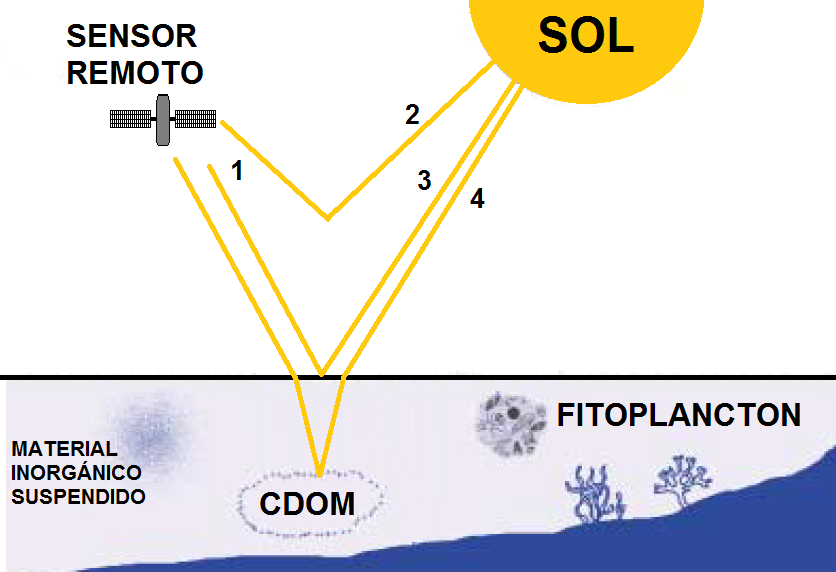
\includegraphics[width=0.8\textwidth]{componentesenelagua}
\caption {Diagrama mostrando los caminos que recorre la luz que llega al sensor (1); (2) la luz
que interactúa con las componentes de la atmósfera (partículas tales como los aerosoles y
moléculas tales como el ozono y el oxígeno); (3) la luz directa que se refleja especularmente en la
superficie del agua; y (4) la luz que emerge del agua y llega al sensor luego de interactuar con las
sustancias presentes en el cuerpo de agua (tales como agua, fitoplancton, partículas, etc.)} 
\label{fig:componentesenelagua}
\end{figure}

El diagrama de la figura \ref{fig:componentesenelagua} simplifica los posibles casos; puesto que no tiene en cuenta situaciones mixtas, como por ej., luz que interactúa con la atmósfera y luego es reflejada por la superficie y finalmente arriba al sensor. Esto no quiere decir que estos casos no deban ser tenidos en cuenta; sino que se omiten del esquema por simplicidad. El proceso de corrección atmosférica elimina las componentes (2) y (3), que son
considerados como ruido en este contexto y son generados por la dispersión
producida tanto por las moléculas del aire como por las partículas (aerosoles). La
radiación que emerge de la capa superficial del mar, la componente (4), es la única que contiene información sobre las sustancias presentes en el
agua. Las características espectrales de la radiancia que emerge del agua dependen de la absorción y
dispersión de la REM de las distintas componentes que se encuentren dentro de la misma (e.g. materia orgánica disuelta y material particulado en suspensión,
incluyendo las células vivas del fitoplancton, sedimento inorgánico y detrito
particulado).

\subsection{Descomposición de la señal que llega al sensor}
La radiancia total que llega al sensor al TOA ($L_{TOA}$) también
puede expresarse en forma equivalente como la reflectancia al tope de la
atmósfera o total, $\rho_{TOA}$, según

\begin{equation}
\rho_{TOA}=\frac{\pi L_{TOA}}{E_{S}\mu_{S}}
\label{rhovsL}
\end{equation}

donde $L_{TOA}$ es la radiancia total medida por el sensor ((1) en la figura \ref{fig:componentesenelagua}), $E_{S}$ es la
irradiancia solar extraterrestre y $\mu_{S}$ es el coseno del ángulo cenital solar ($\ts$).
La reflectancia total, a una determinada longitud de onda $\l$, puede escribirse como
la suma de varias componentes:

\begin{align}
\rho_{TOA}&=\rho_{RAY}+\rho_{AER}+\rho_{R-A}+t[(1-f)\rho_{W}+f\rho_{WC}]+T\rho_{G}\\
&=\rho_{2}+\rho_{3}+\rho_{4}
\label{rhotoaDESCOMP}
\end{align}

siendo

\begin{align}
\rho_{2}&=\rho_{RAY}+\rho_{AER}+\rho_{R-A}\\
\rho_{3}&=t.f\rho_{WC}+T\rho_{G}\\
\rho_{4}&=t.(1-f)\rho_{W}
\label{rho2}
\end{align}

las diferentes componentes esquematizadas en la Fig. \ref{fig:componentesenelagua}. La reflectancia $\rho_{2}$ está compuesta por $\rho_{RAY}$, resultante de procesos de dispersión múltiple por moléculas de aire en ausencia de aerosoles (dispersión Rayleigh); $\rho_{AER}$, el caso contrario (por aerosoles en ausencia de aire), y $\rho_{R-A}$, el término que representa fotones que sufren procesos de dispersión tanto por moléculas de aire como por aerosoles y logran arribar al sensor.
La componente $\rho_{3}$ contiene a $\rho_{G}$, la reflectancia superficial especular directa (\textit{sunglint}), multiplicada por $T$, la transmitancia directa de la atmósfera; y $\rho_{3}$ la reflectancia debida a la espuma, multiplicada por la transmitancia difusa de la atmósfera, $t$, y la fracción de la superficie del mar cubierta por espuma, $f$.
Es apropiado utilizar la transmitancia difusa ($t$) para la reflectancia proveniente del agua ($\rho_{W}$) y de la espuma del mar ($\rho_{WC}$) debido a que ambas tienen una distribución angular
casi uniforme (isótropa), mientras que la reflectancia debida a la reflexión
especular ($\rho_{G}$) es principalmente direccional (anisótropa) y se utiliza la
transmitancia directa ($T$).
Finalmente, la componente $\rho_{4}$, es decir, la que posee información sensible acerca de las sustancias que se hallan en el agua, es la reflectancia debida a fotones que atraviesan la interfase agua-aire y que logran emerger luego a la superficie, medida exactamente sobre la superficie. Nuevamente, para contemplar la posible interacción con la atmósfera, se multiplica por el factor $t$ y por la fracción de la superficie libre de espuma (es decir, $1-f$).

Con el fin de obtener $\rho_{W}$ a partir de la Ec. \ref{rhotoaDESCOMP} se han desarrollado métodos
que permiten calcular los otros términos involucrados o aproximaciones que
permiten simplificarlos. Algunos de estos términos son fácilmente computables o eludibles:

\begin{enumerate}
\item $\rho_{RAY}$ es fácilmente computable, dado que se conocen las propiedades físicas y la distribución de las moléculas de aire en la atmósfera es estable; aunque pueden incorporarse variaciones medibles sobre este factor debidas a diferentes presiones atmosféricas en superficie o concentración de $CO_{2}$, entre otras \cite{bodhaine}.
\item $\rho_{WC}$ y $f$, es decir, las propiedades ópticas y la abundancia de la espuma en el océano, son computables a partir de modelos empíricos, los cuales dependen de la intensidad del viento en superficie \cite{koepke}. Esta, a su vez, puede ser obtenida globalmente a partir de modelos de reanálisis.
\item $\rho_{G}$ afecta a regiones específicas de las imágenes que pueden ser eludidas inclinando el ángulo de visión del sensor (mecanismo disponible para el sensor SeaWIFS a bordo del satélite OrbView-2) o bien removidas de la imagen (única posibilidad para sensores sin este mecanismo, como por ej., el MODIS a bordo del satélite Aqua). Al eludir esta componente, no será necesario tampoco el cálculo de la transmitancia directa, $T$.
\end{enumerate}

El factor de transmitancia difusa de la atmósfera, $t$, depende de la absorción y la dispersión de los fotones que provienen del agua debida a las componentes atmosféricas. En este trabajo, se omitirán los efectos debidos a la absorción gaseosa, es decir, aquella asociada a cualesquiera de las componentes de la atmósfera en estado gaseoso. La misma no fue incorporada debido a que su efecto en las bandas utilizadas en el esquema de corrección atmosférica del presente trabajo (en las regiones del infrarrojo cercano (NIR) y de onda corta (SWIR) del espectro) es muy baja. Precisamente, dichas bandas, correspondientes a las del sensor SABIA-Mar, ocupan intencionalmente estas regiones estratégicas del espectro, también denominadas \textit{ventanas atmosféricas} (véase Fig. \ref{fig:transmitancia}). Obsérvese que para la región del visible, en donde se posiciona el resto de las bandas pertinentes a la determinación de las componentes presentes en el agua, la transmitancia es también cercana a la unidad.

\begin{figure}
\centering
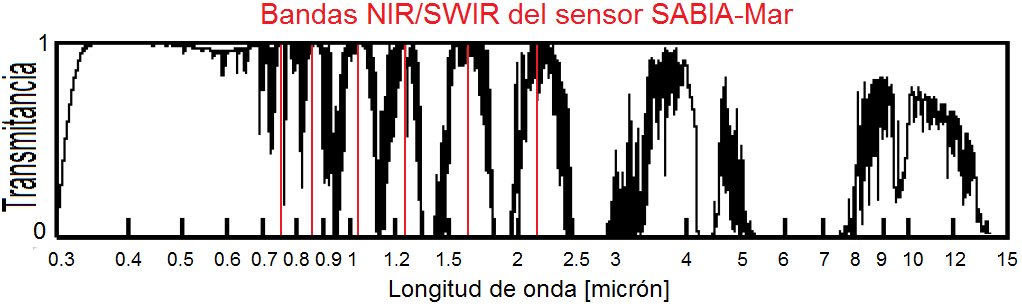
\includegraphics[width=0.8\textwidth]{transmitancia}
\captionof{figure} {Transmitancia asociada con los procesos de absorción en una atmósfera estándar. Se incluyen las bandas de absorción de los siguientes gases: $CO$, $N_{2}O$, $CH_{4}$, $O_{2}$, $O_{3}$, $CO_{2}$ y $H_{2}O$. En rojo, las bandas del sensor SABIA-Mar correspondientes a las regiones NIR y SWIR del espectro electromagnético. Cortesía de Bruce Monger (Cornell/USA).}
\label{fig:transmitancia}
\end{figure}

